\documentclass[a4paper]{article}
\usepackage{import}
\usepackage[utf8]{inputenc}
\usepackage[T1]{fontenc}
\usepackage{textcomp}
\usepackage[italian]{babel}
\usepackage{amsmath, amssymb}
\usepackage{booktabs,xltabular}
\usepackage{amsfonts}
\usepackage{subcaption}
\usepackage{amsthm}
\usepackage{cancel}
\usepackage{mdframed}
\usepackage{makecell}
\usepackage{float}
\usepackage{xcolor}
\usepackage{listings}
\usepackage{gensymb}
\usepackage{graphicx}
\usepackage{bodeplot}
\usepackage{physics}
\usepackage{tikz}
\usetikzlibrary{shapes, arrows, automata, petri, decorations.markings, decorations.pathreplacing, positioning, calc, quotes}
\usepackage{circuitikz}
\usepackage[label=corner]{karnaugh-map}
\graphicspath{{./figures/}}

% Set default font to sans-serif
\renewcommand{\familydefault}{\sfdefault} 
\usepackage{eulervm}

\usepackage{forest}

\usepackage{mathtools}
\DeclarePairedDelimiter\ceil{\lceil}{\rceil}
\DeclarePairedDelimiter\floor{\lfloor}{\rfloor}

% \usepackage{ntheorem}

\usepackage{import}
\usepackage{pdfpages}
\usepackage{transparent}
\usepackage{xcolor}

\usepackage{hyperref}
\hypersetup{
    colorlinks=false,
}

% Code blocks
\definecolor{codegreen}{rgb}{0,0.6,0}
\definecolor{codegray}{rgb}{0.5,0.5,0.5}
\definecolor{codepurple}{rgb}{0.58,0,0.82}
\definecolor{backcolour}{rgb}{0.95,0.95,0.95}

\lstdefinestyle{mystyle}{
	backgroundcolor=\color{backcolour},
	commentstyle=\color{codegreen},
	keywordstyle=\color{magenta},
	numberstyle=\tiny\color{codegray},
	stringstyle=\color{codepurple},
	basicstyle=\ttfamily\footnotesize,
	breakatwhitespace=false,
	breaklines=true,
	captionpos=b,
	keepspaces=true,
	numbers=left,
	numbersep=5pt,
	showspaces=false,
	showstringspaces=false,
	showtabs=false,
	tabsize=2
}

\lstset{style=mystyle}

\usepackage{color}
\usepackage{import}
\usepackage{pdfpages}
\usepackage{transparent}
\usepackage{xcolor}

% Example frame
\theoremstyle{definition}
\newmdtheoremenv[%
	linecolor=gray,leftmargin=0,%
	rightmargin=0,
	innertopmargin=8pt,%
	innerbottommargin=8pt,
	ntheorem]{example}{Esempio}[section]

% Important definition frame
\theoremstyle{definition}
\newmdtheoremenv[%
	linecolor=gray,leftmargin=0,%
	rightmargin=0,
	backgroundcolor=gray!40,%
	innertopmargin=8pt,%
	innerbottommargin=8pt,
	ntheorem]{definition}{Definizione}[section]

% Exercise frame
\theoremstyle{definition}
\newmdtheoremenv[%
	linecolor=gray,leftmargin=0,%
	rightmargin=0,
	innertopmargin=8pt,%
	innerbottommargin=8pt,
	ntheorem]{exercise}{Esercizio}[section]

% Theorem frame
\theoremstyle{definition}
\newmdtheoremenv[%
  linecolor=gray,leftmargin=0,%
  rightmargin=0,
  innertopmargin=8pt,%
  innerbottommargin=8pt,
  ntheorem]{theorem}{Teorema}[section]

\theoremstyle{definition}
\newmdtheoremenv[%
  linecolor=white,leftmargin=0,%
  rightmargin=0,
  innertopmargin=8pt,%
  innerbottommargin=8pt,
  ntheorem]{define}{Definizione utile}[section]

% figure support
\usepackage{import}
\usepackage{xifthen}
\pdfminorversion=7
\usepackage{pdfpages}
\usepackage{transparent}
\newcommand{\incfig}[1]{%
	\def\svgwidth{\columnwidth}
	\import{./figures/}{#1.pdf_tex}
}

% FSM tikz
\tikzset{
    place/.style={
        circle,
        thick,
        draw=black,
        minimum size=6mm,
    },
        state/.style={
        circle,
        thick,
        draw=black,
        fill=white,
        minimum size=6mm,
    },
}

\pdfsuppresswarningpagegroup=1

\usepackage{pgfplots}
\pgfplotsset{compat=1.18,width=10cm}

% Save plots as pdf and reuse them without compiling every time
\usetikzlibrary{external}
\tikzexternalize[prefix=figures/tikz/, optimize=false]


\begin{document}

\begin{titlepage}
	\begin{center}
		\vspace*{1cm}

		\Huge
		\textbf{Probabilità e Statistica\\Esercizi}

		\vspace{0.5cm}
		\LARGE
		UniVR - Dipartimento di Informatica

		\vspace{1.5cm}

		\textbf{Fabio Irimie}

		\vfill


		\vspace{0.8cm}


		2° Semestre 2023/2024

	\end{center}
\end{titlepage}


\tableofcontents
\pagebreak

\section{Introduzione}

\subsection{Interazione con l'utente}
Un modo per far interagire l'utente con il programma è l'interfaccia grafica. L'interazione
può essere ottenuta in vari modi, ad esempio:
\begin{itemize}
    \item Finestre di dialogo
    \item Realtà virtuale
    \item Realtà aumentata
    \item Giochi
\end{itemize}

\subsection{Sintesi e analisi}
La sintesi è il processo di creazione di un'immagine a partire da una descrizione matematica,
mentre l'analisi è il processo di estrazione di informazioni da un concetto già esistente.

\section{Modeling}
La modellazione 3D è un processo di \textbf{descrizione} di un oggetto o una scena al fine
di poterla disegnare. La descrizione avviene attraverso:
\begin{itemize}
  \item \textbf{Struttura}: Viene descritta dalla geometria degli oggetti e dalla loro
    posizione reciproca nello spazio tridimensionale
    \begin{itemize}
      \item Definizione geometrica
      \item Trasformazioni 3D
    \end{itemize}

  \item \textbf{Apparenza}: Descrive come la superficie del modello interagisce con
    la luce (colori, riflessi, ecc...)
    \begin{itemize}
      \item Definizione telecamere virtuali
      \item Definizione sorgenti di luce
      \item Definizione proprietà dei materiali
    \end{itemize}
\end{itemize}

\subsection{Definizione geometrica}
Ci sono varie tecniche di modellazione:
\begin{itemize}
  \item \textbf{Low poly diretta}, ad esempio con Wings3D. È la costruzione manuale di una mesh
    poligonale a bassa risoluzione, partendo anche da primitive già fatte.
  \item \textbf{Subdivision surfaces}, ad esempio con Blender. Si parte da una mesh
    poligonale a bassa risoluzione e si applicano algoritmi di suddivisione per
    ottenere superfici più lisce e dettagliate.
  \item \textbf{Digital sculpting}, ad esempio con ZBrush
  \item \textbf{Modellazione procedurale}, ad esempio con Houdini. Si utilizzano algoritmi
    e regole per generare automaticamente modelli 3D complessi, ad esempio generazione di
    terreni, vegetazione, edifici, ecc...
\end{itemize}

\subsubsection{Mesh}
Gli oggetti tridimensionali vengono codificati come una maglia (mesh) di triangoli.
I triangoli vengono utilizzati perchè sono il poligono più semplice che può essere utilizzato
per approssimare una qualsiasi superficie. Una mesh è composta da:
\begin{itemize}
  \item \textbf{Vertici}: Punti nello spazio 3D
  \item \textbf{Facce}: Insiemi di vertici che formano triangoli
\end{itemize}

\begin{definition}[Definizione matematica di mesh]
  Una mesh di triangoli è una discretizzazione lineare a tratti di una superficie
  continua (un "2-manifold") immersa in \( \mathbb{R}^3 \), cioè un oggetto bidimensionale
  che si trova in uno spazio tridimensionale. Le componenti sono:
  \begin{itemize}
    \item \textbf{Geometria}: i vertici, ciascuno con coordinate \( (x, y, z) \in \mathbb{R}^3 \)
    \item \textbf{Topologia}: come sono connessi tra loro i vertici, nel caso di una tri-mesh
      ogni faccia è definita da un insieme di tre vertici
  \end{itemize}
\end{definition}

\subsection{Trasformazioni 3D}
Per posizionare e orientare gli oggetti nello spazio 3D, si utilizzano trasformazioni
geometriche, che possono essere rappresentate tramite matrici. Le principali trasformazioni sono:
\begin{itemize}
  \item \textbf{Traslazione}: Spostamento di un oggetto da una posizione a un'altra
  \item \textbf{Rotazione}: Rotazione di un oggetto attorno a un asse specifico
  \item \textbf{Scalatura}: Modifica delle dimensioni di un oggetto lungo gli assi
    X, Y e Z
\end{itemize}

\subsection{Telecamere virtuali}
Per visualizzare una scena 3D su uno schermo 2D, è necessario utilizzare
una telecamera virtuale che definisce il punto di vista da cui viene osservata la scena.
Il problema è che nel passaggio dal 2D al 3D c'è perdita di informazione.

Per definire una telecamera virtuale, sono necessari:
\begin{itemize}
  \item \textbf{View point}: da dove si osserva
  \item \textbf{Look at point}: dove si guarda
  \item \textbf{View direction}: orientamento della telecamera
  \item \textbf{Regole di proiezione}:
    \begin{itemize}
      \item Ortografica: mantiene le proporzioni reali degli oggetti
      \item Prospettica: simula la visione umana, con oggetti
        più lontani che appaiono più piccoli
    \end{itemize}
\end{itemize}

\subsubsection{Proiezione}
Il mondo non è infinito, quindi bisogna definire il \textbf{cono di vista} (frustum),
che delimita la porzione di scena visibile dalla telecamera. Il frustum è definito
dal parallelepipedo delimitato da due piani:
\begin{itemize}
  \item \textbf{Near plane}: piano più vicino alla telecamera
  \item \textbf{Far plane}: piano più lontano dalla telecamera
\end{itemize}
Gli oggetti al di fuori del frustum non vengono proiettati (fase di clipping). La proiezione
avviene su un piano di vista (view plane), che rappresenta lo schermo 2D.

\subsection{Illuminazione}
Tramite l'illuminazione si riesce a distinguere la forma degli oggetti tridimensionali.
La modellazione delle luci della scena si occupa del loro posizionamento e del tipo di luce
utilizzata. I tipi di luce più comuni sono:
\begin{itemize}
  \item \textbf{Directional light}: luce proveniente da una direzione specifica, simula
    la luce solare
  \item \textbf{Point light}: luce che si propaga in tutte le direzioni da un punto
    specifico, simula una lampadina
  \item \textbf{Spotlight}: luce che si propaga in un cono da un punto specifico,
    simula un faro
  \item \textbf{Ambient light}: luce diffusa che illumina uniformemente tutta la scena,
    senza una direzione specifica
\end{itemize}

\subsection{Proprietà dei materiali}
Il materiale di cui è fatta la superficie di un oggetto condiziona il suo aspetto nel
momento in cui viene colpito dalla luce. Le proprietà principali dei materiali sono:
\begin{itemize}
  \item \textbf{Colore}
  \item \textbf{Riflettività}
  \item \textbf{Rugosità}
\end{itemize}

\section{Rendering}
Il rendering ha l'obiettivo di creare un'\textbf{immagine bidimensionale} a partire dalla
descrizione di una scena tridimensionale. Ogni pixel dell'immagine deve avere un colore
che dipende dalla geometria, dall'illuminazione e dalle proprietà dei materiali della
scena. Per renderizzare una scena c'è bisogno di tradurre il processo fisico della luce
in un algoritmo e questo ha bisogno di molte semplificazioni e approssimazioni.

\subsection{Modello fisico dell'illuminazione}
La luce è una radiazione elettromagnetica con lunghezza d'onda tra i 400 e i 700 nm che
parte da una \textbf{sorgente} verso un \textbf{ricevente}. La sorgente può essere
un \textbf{emittente} (sorgente primaria) oppure un \textbf{riflettore} (sorgente secondaria).
La lunghezza d'onda determina il colore della luce percepita dall'occhio umano:
\begin{itemize}
  \item Luce monocromatica: Quando è presente soltanto una lunghezza d'onda (es.
    laser)

  \item Luce policromatica: Quando sono presenti più lunghezze d'onda (es. luce solare)
\end{itemize}
L'energia trasportata dalla luce determina l'\textbf{intensità} luminosa.

\subsubsection{Interazione della luce con i materiali}
La luce può interagire con la materia in vari modi:
\begin{itemize}
  \item Una sorgente di luce (luce \textbf{incidente}) illumina la superficie di un oggetto
  \item Una parte della luce \textbf{riflessa} da un punto si distribuisce uniformemente in
    tutte le direzioni (luce \textbf{diffusa})
  \item Una parte della luce viene \textbf{riflessa} da un punto verso una direzione preferita
    (luce \textbf{speculare})
  \item Una parte della luce viene assorbita all'interno del materiale (luce \textbf{trasmessa})
\end{itemize}
Per generare l'immagine bisogna tenere conto della \textbf{quantità di luce} che viene
trasportata fino all'osservatore (camera virtuale) interagendo con i vari materiali.
Il pixel dell'immagine misura dunque la \textbf{radianza} o \textbf{luminanza} delle
superfici visibili dalla camera virtuale.
\begin{itemize}
  \item Fissata la camera virtuale e fissato un pixel si osserva una porzione di superficie
    di un oggetto della scena
  \item Il pixel prende un valore sulla base dello stato fotometrico di questa porzione di
    superficie.
\end{itemize}

\subsection{Equazione del rendering}
Per poter modellare al meglio i fenomeni fotometrici dei materiali viene definita la 
\textbf{Bidirectional Reflectance Distribution Function} (BRDF), che descrive come la luce
viene riflessa da una superficie in funzione della direzione di arrivo e della direzione
di uscita della luce:
\[
  f_r(x, \omega_i, \omega_o)
\] 
Dove:
\begin{itemize}
  \item \( x \) è il punto della superficie
  \item \( \omega_i \) è l'angolo della luce incidente
  \item \( \omega_o \) è l'angolo della luce riflessa
\end{itemize}

\subsubsection{Path tracing}
Il path tracing è un algoritmo di rendering che simula il comportamento della luce
nella scena tracciando il percorso dei raggi di luce. Al posto di calcolare quali raggi
partendo dalla sorgente di luce colpiscono la camera, si parte dalla camera e si
tracciano i raggi che da essa colpiscono la fonte di luce. Questo metodo è più efficiente
perchè si concentra solo sui raggi che effettivamente contribuiscono all'immagine finale.

\subsubsection{Algoritmi di lighting}
Ci sono diversi metodi per calcolare l'illuminazione in una scena 3D:
\begin{itemize}
  \item I metodi \textbf{locali} tengono conto solo dell'effetto delle sorgenti di luce
    dirette sulla superficie, senza considerare le interazioni tra le superfici.
    Esempi: \textbf{Flat shading}, \textbf{Gouraud shading}, \textbf{Phong shading}
  \item I metodi \textbf{globali} considerano tutte le interazioni della luce con le
    superfici della scena, inclusi riflessi, rifrazioni e ombre. Esempi: \textbf{Ray tracing},
    \textbf{Radiosity}, \textbf{Path tracing}
\end{itemize}

\subsubsection{Shading}
Lo shading ha lo scopo di determinare il colore effettivo dei pixel a partire da un modello
di illuminazione dato. Determina come e quando applicare il modello di illuminazione prescelto.
Ci sono tre tipi principali di shading:
\begin{itemize}
  \item \textbf{Flat shading}: A ogni primitiva geometrica (triangolo) è associato uno
    stesso colore uniforme. È il metodo più semplice e veloce, ma meno realistico.
  \item \textbf{Gouraud shading}: Il valore di illuminazione viene calcolato ai vertici
    e viene \textbf{interpolato} per i pixel (fragment) interni
  \item \textbf{Phong shading}: Vengono interpolate le normali ai vertici per ottenere le
    normali di ciascun pixel e il modello viene calcolato per ogni pixel. Produce risultati
    migliori e più realistici, ma è più costoso computazionalmente.
\end{itemize}

\section{Animazione}
L'animazione in 3D è il processo di creazione di modelli (o camera virtuale)
in movimento all'interno di una scena tridimensionale.

\subsection{Produzione del modello}
Il modello viene costruito con una descrizione geometrica del suo aspetto e in base
al tipo di \textbf{cinematica} adottata per l'animazione è possibile dotare il
modello di una struttura scheletrica (\textbf{rigging}) che ne consente il movimento.

\subsubsection{Rigging}
È la fase di preparazione del modello per fare in modo che possa essere animato. Vengono
inserite delle componenti aggiuntive al modello che permettono all'animazione di
diventare \textbf{parametrica} (cioè dipendente da parametri variabili nel tempo).
L'obiettivo è quello di definire i parametri che governano l'animazione in modo da
inserire una sorta di \textbf{semantica} nel \textbf{movimento}.

\vspace{1em}
\noindent
L'animazione è la fase in cui i parametri definiti dal rigging vengono istanziati per
generare i movimenti e le deformazioni desiderate.

\subsubsection{Animazione del volto}
Per animare un volto umano in modo realistico si può ricomporre il movimento del volto a
partire dal controllo dei movimenti elementari della muscolatura. Questo viene fatto
muovendo gruppi di punti di controllo o interpolando tra una forma di riferimento.
Le tecniche più diffuse sono:
\begin{itemize}
  \item \textbf{Blend based}: si costruiscono numerose versioni del modello
    (dette shape di espressioni di base). L'animazione deriva dalla combinazione
    di queste versioni.
  \item \textbf{Rig based}: si inseriscono delle "ossa" all'interno della faccia che
    controllano i movimenti e li propagano sulla superficie del volto.
  \item \textbf{Phisycally based}: vengono simulate le proprietà fisice ed elastiche dei tessuti
    molli della pelle e deu muscoli.
\end{itemize}

\subsubsection{Animazione del corpo umano}
L'animazione del corpo umano consiste nella creazione di un modello geometrico articolato,
cioè un manichino. Per animare il manichino si devono definire:
\begin{itemize}
  \item Parametri fisici della struttura articolata
  \item Tipologie standard di comportamento
  \item Interazione con l'ambiente circostante
  \item Aspetto del manichino
\end{itemize}
Un esempio di modello di struttura articolata è lo \textbf{stick figure}, cioè aste
rigide collegate con giunti in grado di ruotare l'uno rispetto all'altro. Questo simula
uno scheletro umano semplificato.

\vspace{1em}
\noindent
Le parti di una struttura articolata sono organizzate in una gerarchia ad albero, dove
ogni nodo rappresenta una parte del corpo e le trasformazioni applicate a un nodo
vengono \textbf{propagate} ai nodi figli.

\subsubsection{Animazione automatica}
Animare in 3D con metodi informatici significa attribuire variazioni ai valori assunti dai
parametri che descrivono l'aspetto e lo stato di un oggetto nella scena 3D.
Si crea qundi una funzione parametrica che varia nel tempo. Ci sono due approcci principali:
\begin{itemize}
  \item \textbf{Traiettoria analitica}: Si definisce una funzione matematica che descrive il
    movimento dell'oggetto nel tempo. Ad esempio, una traiettoria circolare può essere
    descritta con funzioni trigonometriche.
  \item \textbf{Keyframing}: Si definiscono dei fotogrammi chiave (keyframe) che rappresentano
    stati specifici dell'oggetto in determinati istanti di tempo. Il software interpola
    automaticamente i valori tra i keyframe per creare un'animazione fluida. Il tipo
    di interpolazione può essere lineare, cubica, spline, ecc...
\end{itemize}

\vspace{1em}
\noindent
Un modo alternativo per definire delle traiettorie complesse è l'utilizzo di
\textbf{motion capture}, che consiste nel registrare i movimenti di un attore reale
e trasferirli a un modello 3D.

\section{Graphics Pipeline}
La graphics pipeline è il processo che trasforma una scena 3D in un'immagine 2D visualizzabile
su uno schermo. Tra il "mondo" 3D e il "mondo" 2D bisogna introdurre delle trasformazioni
intermedie per poter rappresentare correttamente la scena.
\begin{figure}[H]
  \centering
  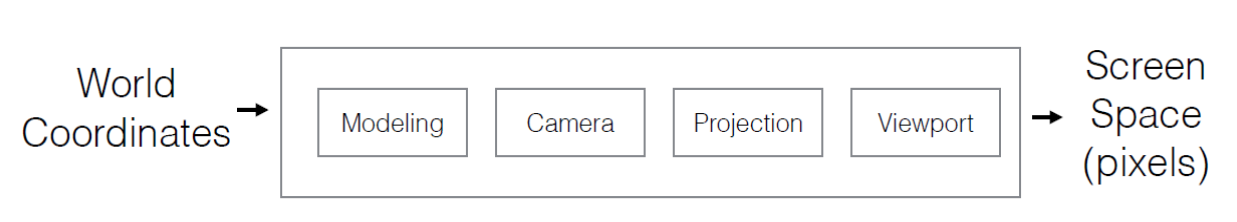
\includegraphics[width=0.9\textwidth]{trasformazioni}
  \caption{Trasformazione della scena 3D in immagine 2D}
\end{figure}
\noindent
Per applicare queste trasformazioni bisogna avere un sistema di coordinate ben definito
in ogni fase della pipeline:
\begin{itemize}
  \item \textbf{Object coordinates}: coordinate locali dell'oggetto
  \item \textbf{World coordinates}: coordinate globali della scena
  \item \textbf{Camera coordinates}: coordinate relative alla telecamera virtuale
  \item \textbf{Screen coordinates}: coordinate 2D dell'immagine finale
\end{itemize}
\begin{figure}[H]
  \centering
  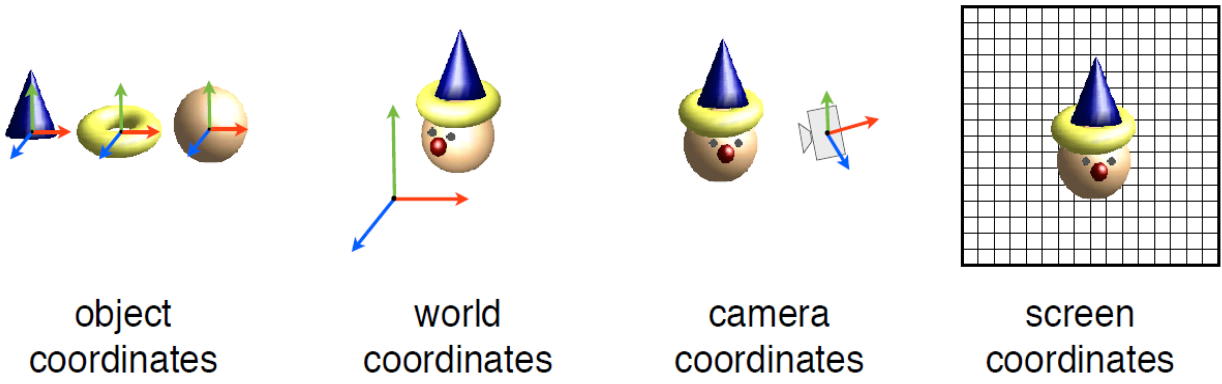
\includegraphics[width=0.9\textwidth]{coordinate}
  \caption{Sistemi di coordinate nella graphics pipeline}
\end{figure}

\subsection{Trasformazioni}
Per realizzare la pipeline grafica bisogna capire il processo che mappa le componenti
della scena da uno spazio di coordinate ad un altro. Le trasformazioni principali sono:
\begin{figure}[H]
  \centering
  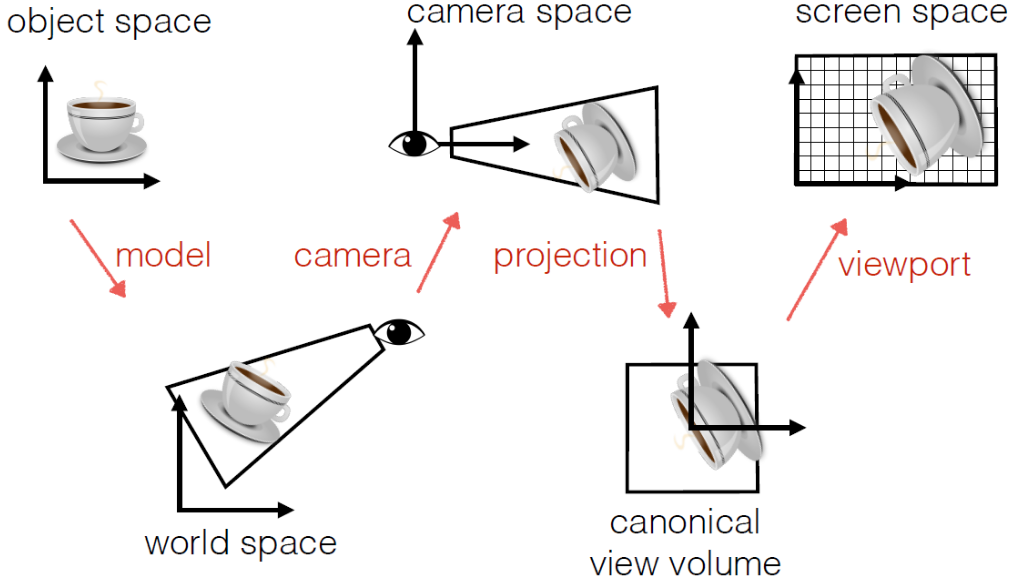
\includegraphics[width=0.9\textwidth]{trasformazioni_pipeline}
  \caption{Trasformazioni nella graphics pipeline}
\end{figure}

\subsubsection{Model transformation}
La model transformation mappa le coordinate locali dell'oggetto (object coordinates)
nelle coordinate globali della scena (world coordinates) in base al grafo della scena.
Questa trasformazione tiene conto della posizione, dell'orientamento e della scala
dell'oggetto nella scena.
\begin{figure}[H]
  \centering
  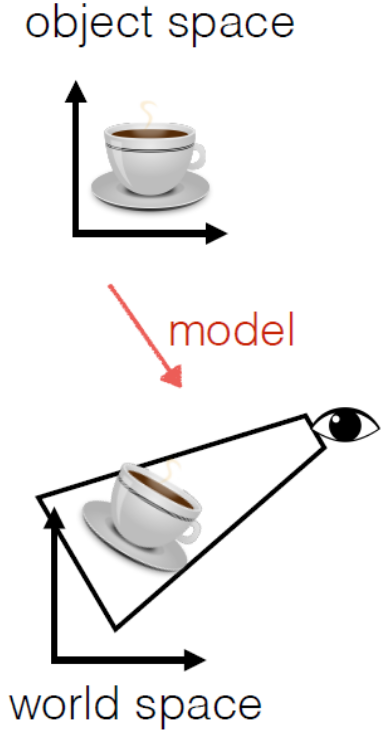
\includegraphics[width=0.3\textwidth]{model_transformation}
  \caption{Model transformation}
\end{figure}

\subsubsection{Camera transformation}
La camera transformation mappa le coordinate globali della scena (world coordinates)
nelle coordinate relative alla telecamera virtuale (camera coordinates). Questa
trasformazione tiene conto della posizione e dell'orientamento della telecamera
nella scena. Questa trasformazione dipende soltanto dalla posizione della telecamera.
\begin{figure}[H]
  \centering
  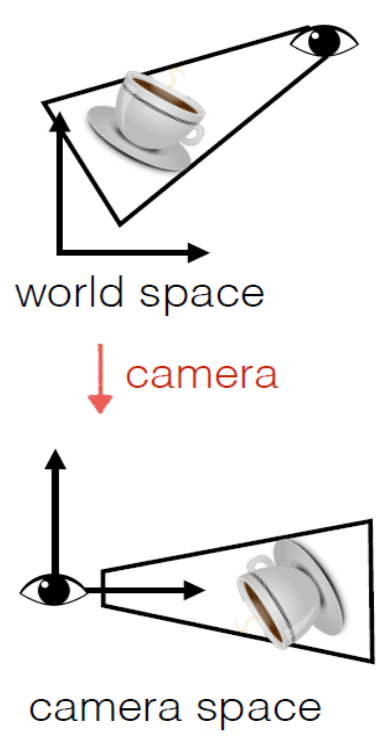
\includegraphics[width=0.3\textwidth]{camera_transformation}
  \caption{Camera transformation}
\end{figure}

\subsubsection{Projection transformation}
La projection transformation mappa le coordinate della telecamera (camera coordinates)
nelle coordinate normalizzate del dispositivo (clip space),
cioè uno spazio di coordinate 3D normalizzato in cui le coordinate X e Y sono comprese
tra -1 e 1.
\begin{figure}[H]
  \centering
  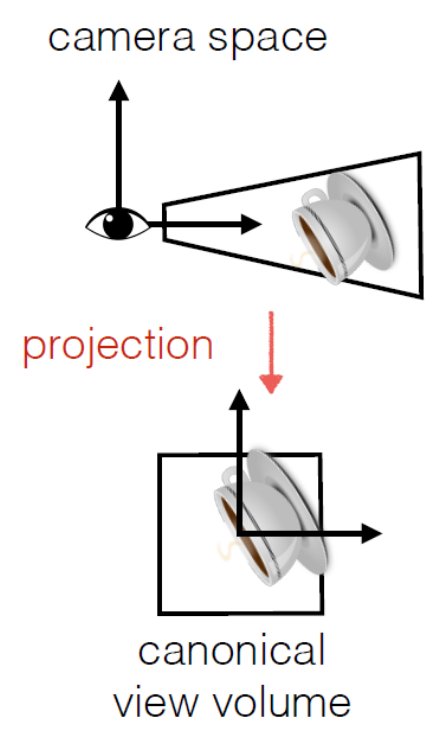
\includegraphics[width=0.3\textwidth]{projection_transformation}
  \caption{Projection transformation}
\end{figure}
La coordinata Z dipende dal tipo di proiezione (ortografica o prospettica).
\begin{figure}[H]
  \centering
  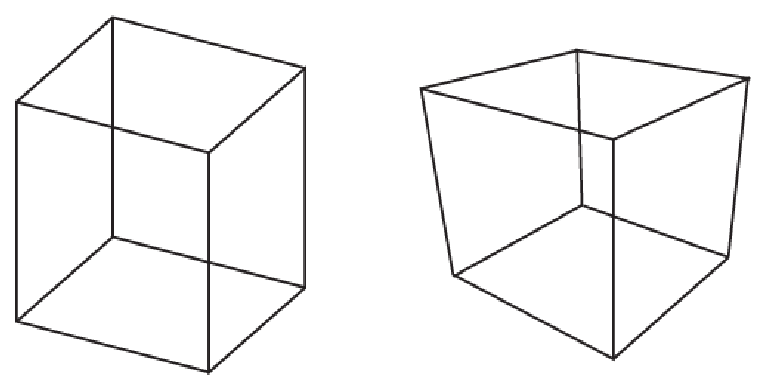
\includegraphics[width=0.4\textwidth]{prospettive}
  \caption{Proiezione ortografica (sinistra) e prospettica (destra)}
\end{figure}

\subsubsection{Viewport transformation}
La viewport transformation mappa le coordinate normalizzate del dispositivo (clip space)
nelle coordinate dello schermo (screen coordinates), cioè le coordinate 2D dell'immagine
finale. Dipende soltanto dalla risoluzione dello schermo.
\begin{figure}[H]
  \centering
  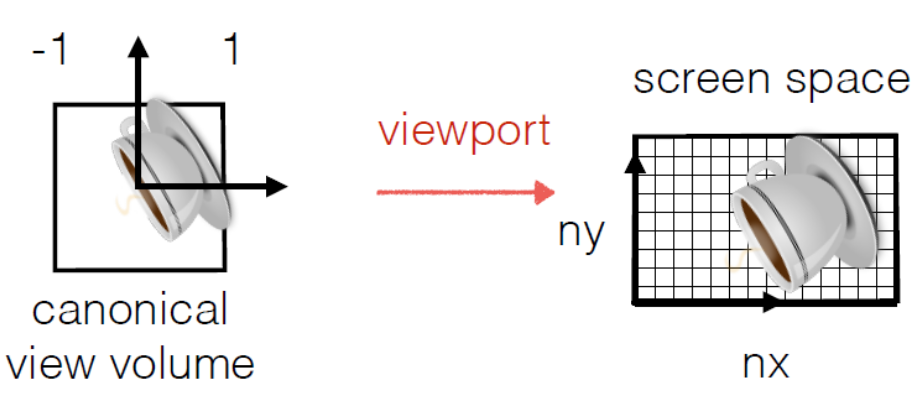
\includegraphics[width=0.6\textwidth]{viewport_transformation}
  \caption{Viewport transformation}
\end{figure}

\subsection{Pipeline}
La sequenza di operazioni richiesta per trasformare gli oggetti di una scena in pixel
su uno schermo è chiamata \textbf{graphics pipeline}. Ci sono due tipi di pipeline:
\begin{itemize}
  \item \textbf{Hardware pipeline}: utilizza la GPU tramite API grafiche come OpenGL
    o Direct3D
  \item \textbf{Software pipeline}: implementa tutte le fasi della pipeline tramite codice
    eseguito dalla CPU
\end{itemize}
Le fasi principali della graphics pipeline sono:
\begin{enumerate}
  \item \textbf{Input}: Gli oggetti della scena, sempre descritti da triangoli, vengono
    passati alla pipeline
  \item \textbf{Vertex processing}: Ogni vertice dei triangoli viene trasformato dalle
    coordinate locali (object coordinates) alle coordinate della telecamera (camera coordinates)
    tramite la model transformation e la camera transformation.
  \item \textbf{Rasterization}: I triangoli vengono convertiti in insiemi di pixel (fragments)
  \item \textbf{Fragment processing}: Per ogni pixel viene calcolato il colore in base
    al modello di illuminazione scelto e alle proprietà dei materiali.
  \item \textbf{Fragment blending}: I pixel vengono scritti nel framebuffer per creare
    l'immagine finale
\end{enumerate}
\begin{figure}[H]
  \centering
  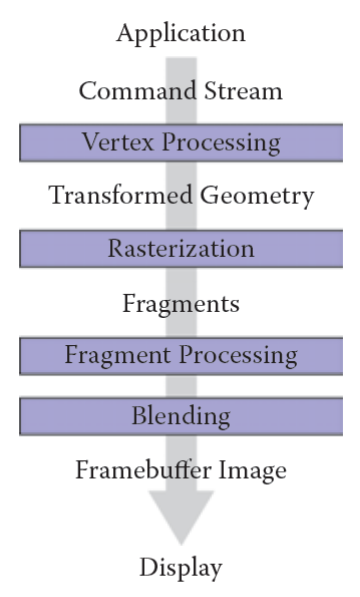
\includegraphics[width=0.4\textwidth]{graphics_pipeline}
  \caption{Fasi della graphics pipeline}
\end{figure}
Il programmatore può intervenire in due fasi della pipeline (viola nell'immagine):
\begin{itemize}
  \item \textbf{Vertex shader}: Permette di personalizzare il processo di trasformazione
    dei vertici
  \item \textbf{Fragment shader}: Permette di personalizzare il processo di calcolo del colore
    dei pixel
\end{itemize}
\begin{figure}[H]
  \centering
  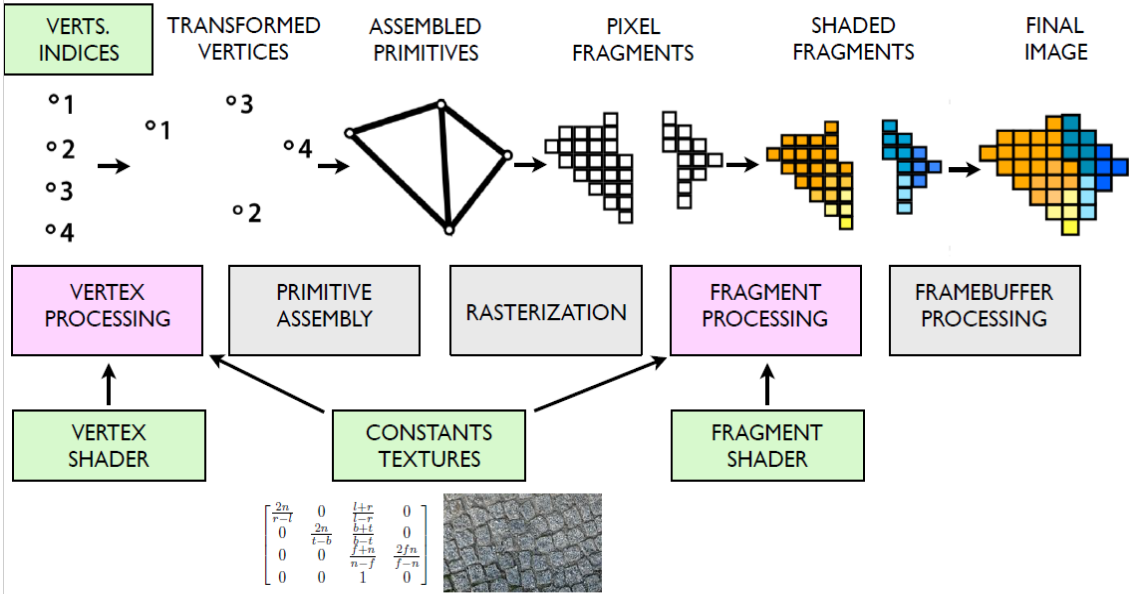
\includegraphics[width=1\textwidth]{graphics_pipeline_example}
  \caption{Esempio di graphics pipeline}
\end{figure}


\subsubsection{Rasterization}
La rasterization è il processo di conversione delle primitive geometriche (di solito
triangoli) in pixel sull'immagine 2D.
\begin{figure}[H]
  \centering
  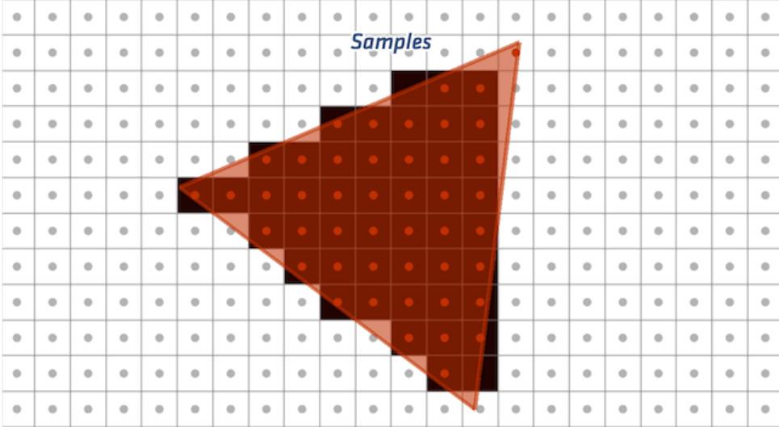
\includegraphics[width=0.6\textwidth]{rasterization}
  \caption{Rasterization}
\end{figure}
\noindent
Durante la rasterization, ogni triangolo viene suddiviso in pixel e per ogni pixel
viene calcolato se disegnarlo oppure no.
\vspace{1em}
\noindent
Quando il rasterizer riceve una primitiva esegue questi passi:
\begin{enumerate}
  \item \textbf{Enumera} i pixel coperti dalla primitiva
  \item \textbf{Interpola} i valori dei vertici (coordinate, colori, normali, ecc...),
    chiamati attributi, per ogni pixel della primitiva
\end{enumerate}
L'output del rasterizer è un insieme di \textbf{fragments}, uno per ogni pixel, che
copre tutta l'area della primitiva. Ogni fragment si trova in un pixel specifico dello
schermo e contiene il suo insieme di attributi.

\vspace{1em}
\noindent
\begin{itemize}
  \item 
    Prima che una primitiva venga rastereizzata, i vertici che la definiscono devono essere
    trasformati in coordinate screen space e i colori e altri eventuali attributi devono
    essere noti. Questo viene effettuato dalla fase di \textbf{vertex processing}. Anche
    gli attributi devono essere trasformati in clip space.

  \item Dopo aver rasterizzato si svolgono altri processi sui fragment, come il calcolo
    del colore o della profondita e viene svolto dalla fase di \textbf{fragment processing}.
\end{itemize}


\subsubsection{Rasterization di linee}
Per rasterizzare una linea tra due punti \( (x_0, y_0) \) bisogna rappresentarla come
un rettangolo per fornire uno spessore alla linea. Si disegnano tutti i pixel che hanno
il centro all'interno del rettangolo.
\begin{figure}[H]
  \centering
  \begin{minipage}{0.48\textwidth}
     \centering
     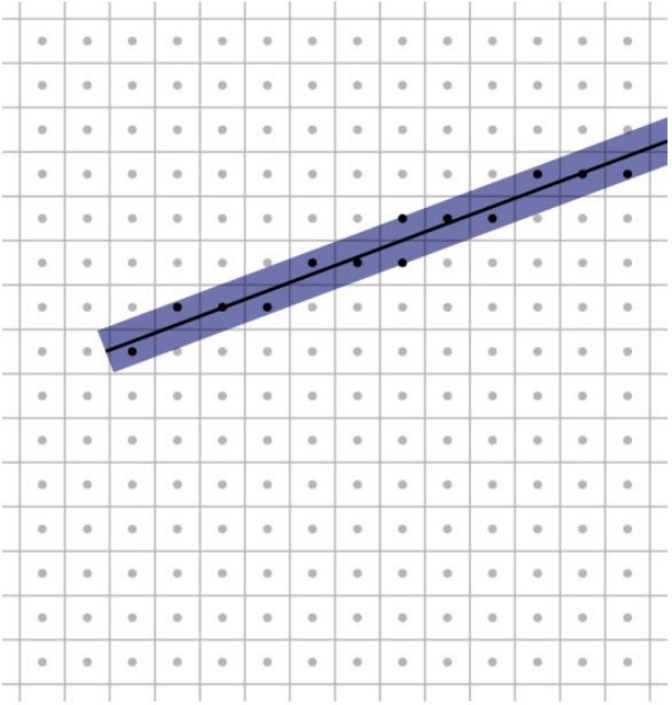
\includegraphics[width=.9\linewidth]{raster_line}
     \caption{Rasterization di una linea}
   \end{minipage}\hfill
   \begin{minipage}{0.48\textwidth}
     \centering
     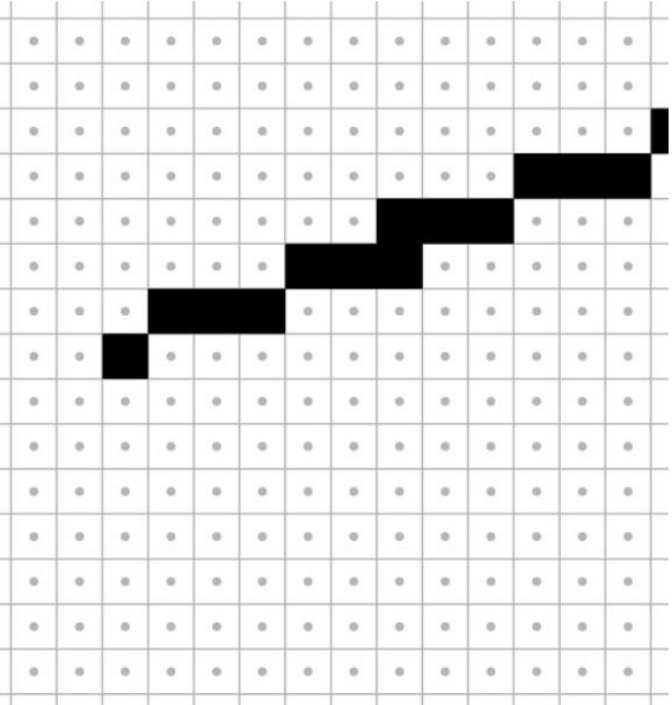
\includegraphics[width=.9\linewidth]{raster_line_2}
     \caption{Output della rasterization di una linea}
   \end{minipage}
\end{figure}
\noindent
Si può migliorare l'approssimazione utilizzando l'algoritmo \textbf{Mid-Point}
che seleziona i pixel in modo da minimizzare l'errore tra la linea ideale e la
linea rasterizzata. Consideriamo l'equazione implicita di una linea tra due punti:
\[
  f(x,y) = (y_0 - y_1)x + (x_1 - x_0)y + (x_0y_1 - x_1y_0) = 0
\] 
L'algoritmo (solo per le linee della griglia orizzontali) è il seguente:
\begin{lstlisting}[language=Python]
y = y_0
for x = x_0 to x_1:
    draw(x, y)

    if f(x + 1, y + 0.5) < 0:
        y = y + 1
\end{lstlisting}
L'effetto di questo algoritmo è il seguente:
\begin{figure}[H]
  \centering
  \begin{minipage}{0.48\textwidth}
     \centering
     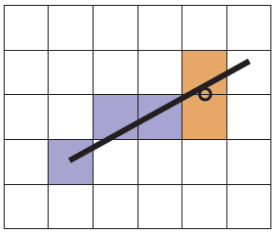
\includegraphics[width=.9\linewidth]{midpoint_line}
     \caption{La linea si trova sopra il midpoint, quindi viene disegnato il pixel in alto}
   \end{minipage}\hfill
   \begin{minipage}{0.48\textwidth}
     \centering
     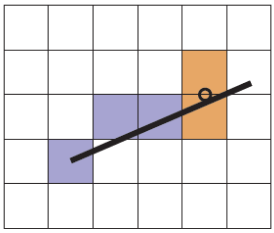
\includegraphics[width=.9\linewidth]{midpoint_line_2}
     \caption{La linea si trova sotto il midpoint, quindi viene disegnato il pixel in basso}
  \end{minipage}
\end{figure}

\subsubsection{Rasterization di triangoli}
Un triangolo è rappresentato come una tripla di coordinate bidimensionali:
\[
  (x_0, y_0), (x_1, y_1), (x_2, y_2)
\] 
\begin{figure}[H]
  \centering
  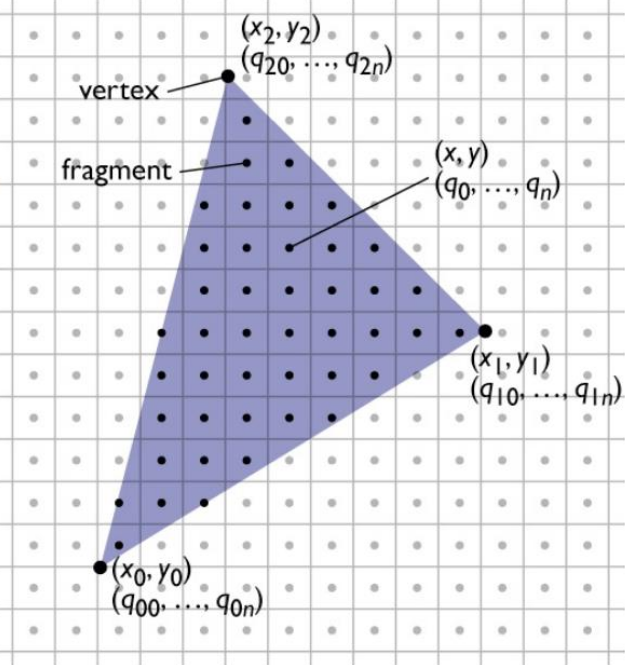
\includegraphics[width=0.6\textwidth]{triangle}
  \caption{Rappresentazione di un triangolo}
\end{figure}
\noindent
Il metodo più utile per rasterizzare un triangolo è usando le
\textbf{coordinate baricentriche}, che permettono di esprimere la posizione di un punto
all'interno del triangolo come combinazione lineare dei vertici del triangolo stesso:
\[
  \begin{aligned}
    x &= \alpha x_0 + \beta x_1 + \gamma x_2 \\
    y &= \alpha y_0 + \beta y_1 + \gamma y_2 \\
    \text{con }& \alpha + \beta + \gamma = 1
  \end{aligned}
\] 
\begin{figure}[H]
  \centering
  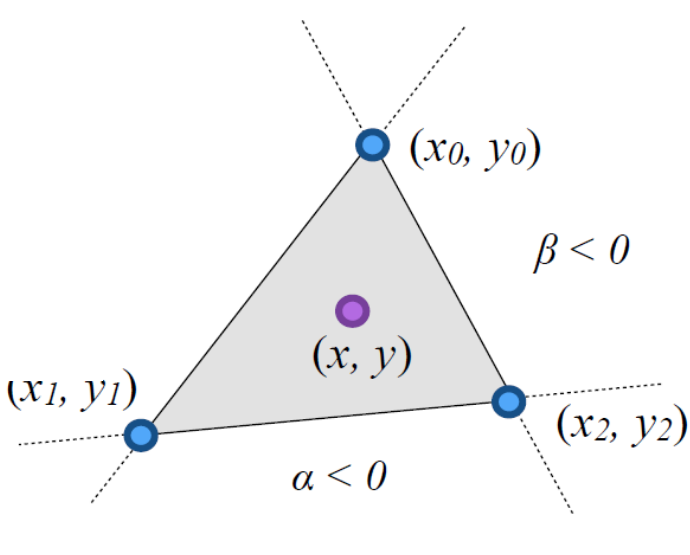
\includegraphics[width=0.6\textwidth]{barycentric}
  \caption{Coordinate baricentriche}
\end{figure}
\noindent
Bisogna quindi calcolare i valori di \( \alpha, \beta, \gamma \) che dipendono dal
triangolo. Consideriamo il seguente triangolo:
\begin{figure}[H]
  \centering
  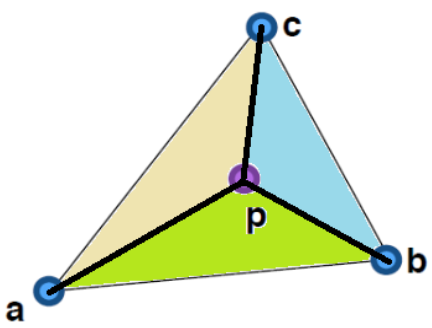
\includegraphics[width=0.4\textwidth]{barycentric2}
  \caption{Triangolo per il calcolo delle coordinate baricentriche}
\end{figure}
\[
  \begin{aligned}
    \alpha(p) = \frac{\color{blue}area(p, b, c)\color{black}}{area(a, b, c)}
    \quad \text{ vale 1 quando } p = a \\
    \beta(p) = \frac{\color{orange}area(a, p, c)\color{black}}{area(a, b, c)}
    \quad \text{ vale 1 quando } p = b \\
    \gamma(p) = \frac{\color{green}area(a, b, p)\color{black}}{area(a, b, c)}
    \quad \text{ vale 1 quando } p = c \\
  \end{aligned}
\] 
La combinazione lineare delle coordinate baricentriche permette di ottenere la posizione
di un qualsiasi fragment all'interno del triangolo, ma anche di interpolare qualsiasi
attributo associato ai vertici del triangolo (colore, normale, coordinate texture, ecc...).
Il codice per rasterizzare un triangolo è il seguente:
\begin{lstlisting}[language=Python]
for all y:
    for all x:
        compute (alpha, beta, gamma) for pixel (x, y)
        if (alpha >= 0 and alpha <= 1 and
          beta >= 0 and beta <= 1 and
          gamma >= 0 and gamma <= 1):
            draw(x, y)
\end{lstlisting}
\begin{figure}[H]
  \centering
  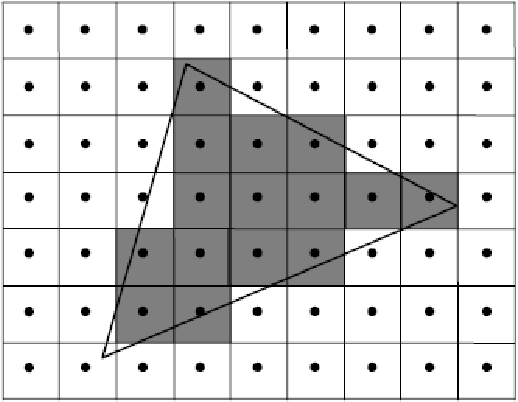
\includegraphics[width=0.6\textwidth]{raster_triangle}
  \caption{Rasterization di un triangolo}
\end{figure}

\vspace{1em}
\noindent
Un esempio di interpolazione del colore ai vertici di un triangolo è il seguente:
\begin{figure}[H]
  \centering
  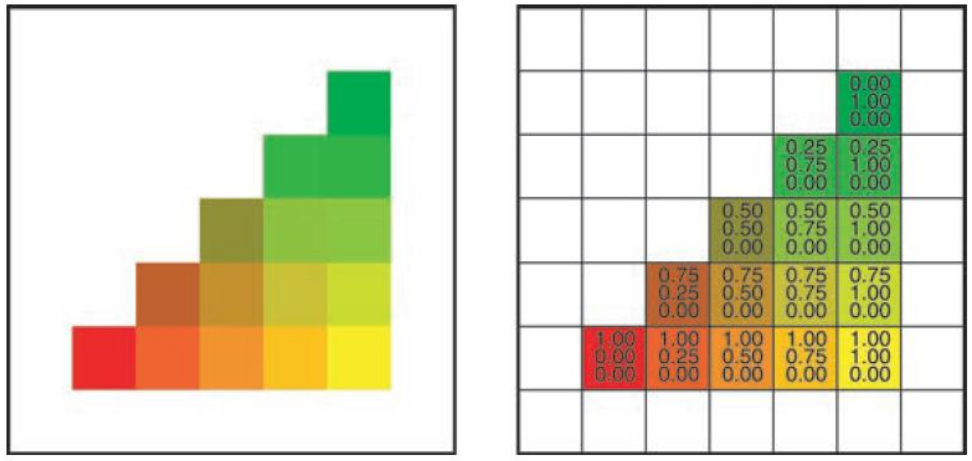
\includegraphics[width=0.8\textwidth]{triangle_color_interpolation}
  \caption{Interpolazione del colore in un triangolo}
\end{figure}

\vspace{1em}
\noindent
Quando si rasterizzano più triangoli bisogna stare attenti a non disegnare più volte
lo stesso pixel:
\begin{figure}[H]
  \centering
  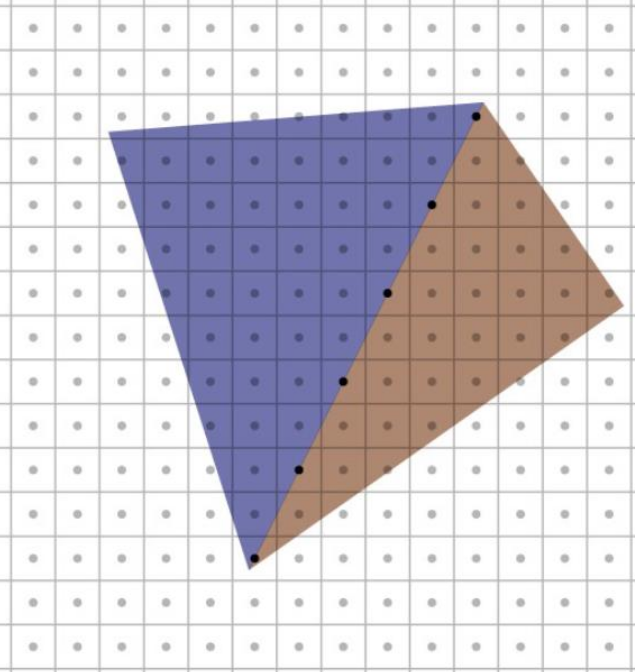
\includegraphics[width=0.6\textwidth]{overlap_triangles}
  \caption{Esempio di overlap tra triangoli}
\end{figure}

\subsubsection{Clipping}
Il clipping è il processo di rimozione delle parti delle primitive geometriche
che si trovano al di fuori dello schermo e al di fuori della camera virtuale. Bisogna
quindi tagliare la parte non visible della primitiva e mantenere solo la parte visibile
modificando eventualmente la sua topologia:
\begin{figure}[H]
  \centering
  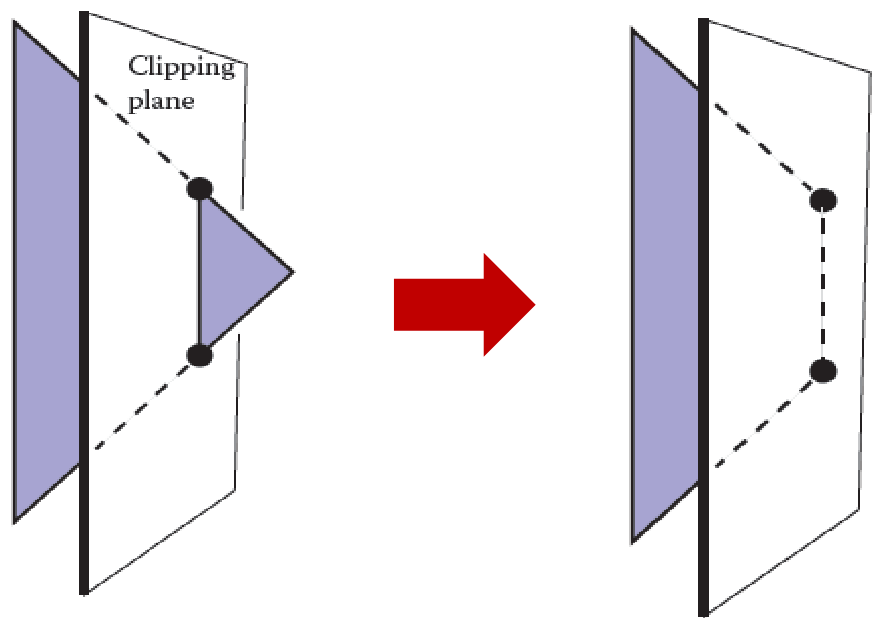
\includegraphics[width=0.7\textwidth]{clipping}
  \caption{Clipping di una primitiva}
\end{figure}

La camera virtuale è rappresentata da un \textbf{frustum}, cioè un volume delimitato
da due piani (near plane e far plane) e da quattro piani laterali (left, right, top, bottom).
La scena è visualizzata soltanto se si trova all'interno del frustum, quindi tra il near
plane e il far plane.

\vspace{1em}
\noindent
Ci sono quattro casi durante un clip:
\begin{itemize}
  \item Tutta la primitiva è dentro il frustum: non serve fare nulla
  \item Tutta la primitiva è fuori dal frustum: si scarta la primitiva
  \item La primitiva è parzialmente dentro il frustum: si calcolano i punti di intersezione
    con i piani del frustum e si crea una nuova primitiva con la parte visibile
  \item La primitiva attraversa più piani del frustum: si calcolano i punti di intersezione
    con tutti i piani del frustum e si crea una nuova primitiva con la parte visibile
\end{itemize}
\begin{figure}[H]
  \centering
  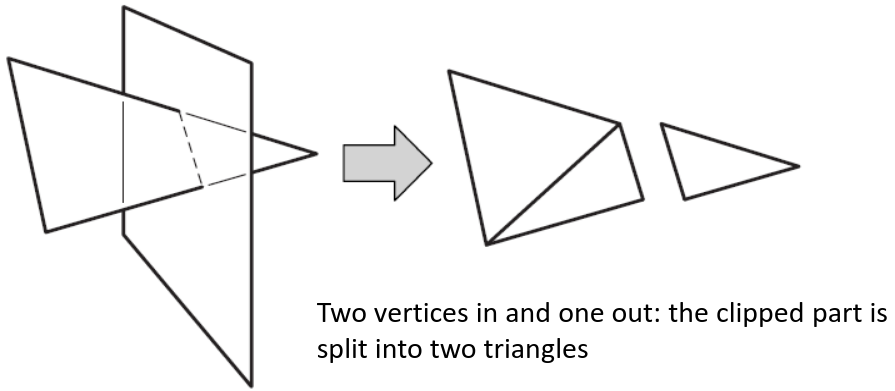
\includegraphics[width=0.7\textwidth]{clipping2}
  \caption{Cambio di topologia dopo il clipping}
\end{figure}

\subsubsection{Intersezione tra una linea e un piano}
Consideriamo l'equazione di un piano:
\[
  f(p) = n \cdot p + D = 0
\] 
dove:
\begin{itemize}
  \item \( n \) è il vettore normale al piano
  \item \( p \) è un punto generico del piano
  \item \( D \) è la distanza del piano dall'origine
\end{itemize}
E l'equazione di una linea:
\[
  p = a + t(b - a)
\] 
dove:
\begin{itemize}
  \item \( a \) e \( b \) sono i due punti estremi della linea che definisce la direzione
  \item \( t \) è un parametro scalare
\end{itemize}
Sostituendo l'equazione della linea in quella del piano si ottiene l'equazione per
calcolare il parametro \( t \) del punto di intersezione:
\[
  n \cdot \left( a + t \left( b-a \right)  \right) + D = 0
\] 
risolvendo per t si ottiene:
\[
  t = \frac{n \cdot a+D}{n \cdot (a-b)}
\] 

\subsubsection{Blending}
La fase di blending combina i fragment generati dalle primitive che si sovrappongono
a ogni pixel per calcolare il colore finale. Questa fase è molto importante per gestire
le occlusioni e per la rimozione delle superfici nascoste (hidden surface removal, HSR).
\begin{figure}[H]
  \centering
  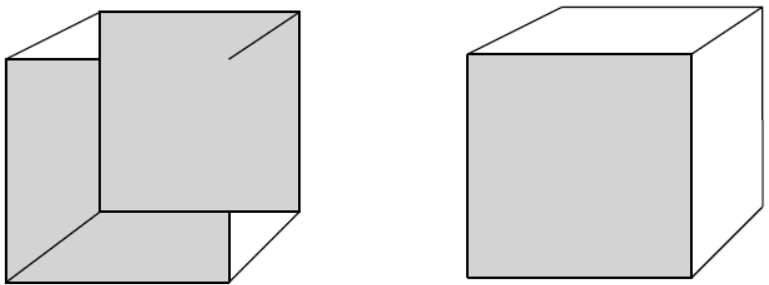
\includegraphics[width=0.6\textwidth]{blending}
  \caption{Blending di fragment sovrapposti}
\end{figure}

\vspace{1em}
\noindent
L'algoritmo di blending più è il \textbf{Painter's algorithm}, disegna per primi i fragment
più lontani e poi quelli più vicini, sovrapponendoli. In questo modo, i fragment più vicini
coprono quelli più lontani.
\begin{figure}[H]
  \centering
  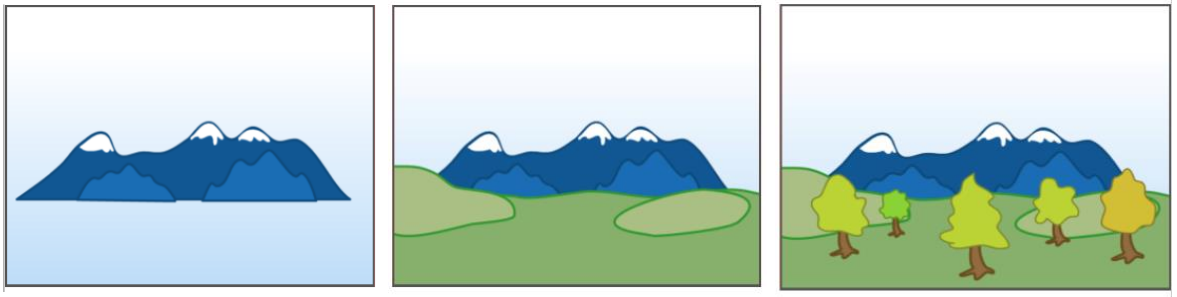
\includegraphics[width=0.6\textwidth]{painter_algorithm}
  \caption{Painter's algorithm}
\end{figure}

\vspace{1em}
\noindent
Un altro metodo per il blending è il \textbf{Z-buffering}, che consiste nel mantenere
una \textbf{depth map} (Z-buffer) che memorizza la profondità di ogni pixel. Se la
profondità del nuovo fragment è minore di quella memorizzata nel Z-buffer, il fragment
viene disegnato e la profondità viene aggiornata, altrimenti viene scartato.
\begin{figure}[H]
  \centering
  \begin{minipage}{0.48\textwidth}
     \centering
     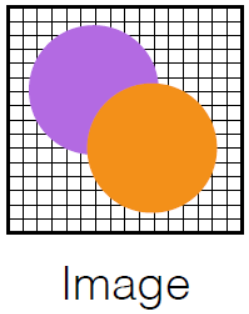
\includegraphics[width=.9\linewidth]{z_buffer}
     \caption{Buffer dell'immagine}
   \end{minipage}\hfill
   \begin{minipage}{0.48\textwidth}
     \centering
     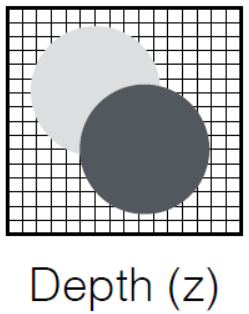
\includegraphics[width=.9\linewidth]{z_buffer2}
     \caption{Buffer della profondità}
   \end{minipage}
\end{figure}
Per rappresentare la profondità di solito più un pixel è scuro più è vicino alla camera.
Un esempio di Z-buffering è il seguente:
\begin{figure}[H]
  \centering
  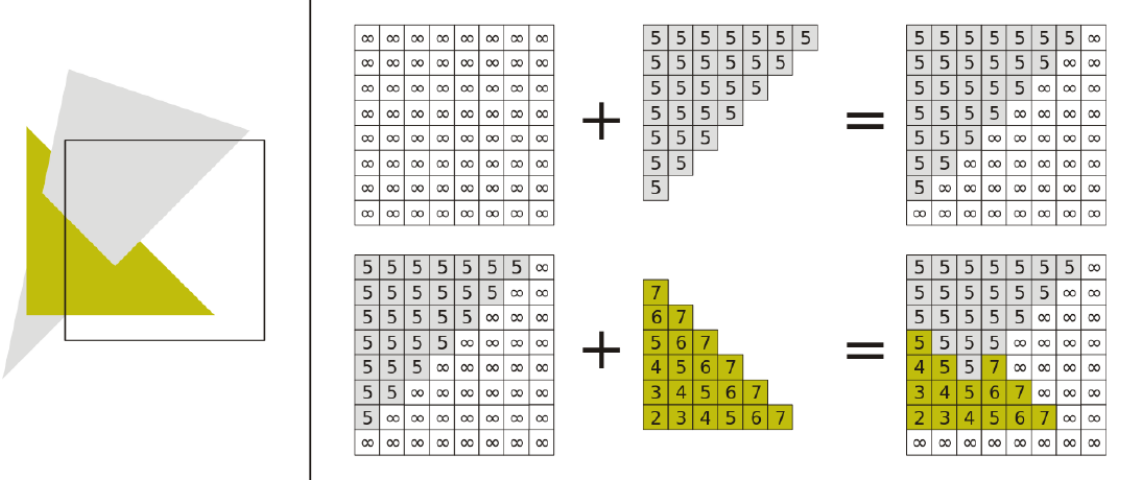
\includegraphics[width=0.6\textwidth]{z_buffering_example}
  \caption{Esempio di Z-buffering}
\end{figure}

\vspace{1em}
\noindent
Siccome il buffer della profondità ha una risoluzione limitata, possono verificarsi
dei problemi di \textbf{Z-fighting}, cioè due fragment molto vicini tra loro che
creano artefatti visivi nell'immagine finale:
\begin{figure}[H]
  \centering
  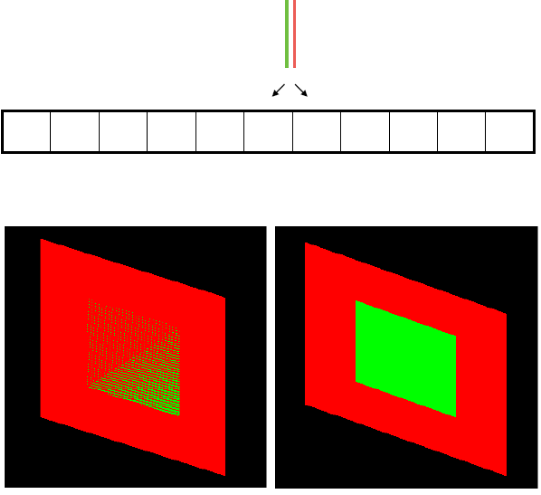
\includegraphics[width=0.6\textwidth]{z_fighting}
  \caption{Esempio di Z-fighting}
\end{figure}


\end{document}
